%=====================================================================
\section{Passive ovals and ellipses}\label{sec:spassive}
Passive references of the shapes used in the active comparison (P5, $k=6$: the four small ovals and the three ellipses), the
pinched ovals (P2, P3) and the validation shapes (T2). Galleries: top rows of Figs.~\ref{fig:maps-small} and \ref{fig:maps-ell},
and the last two panels of Fig.~\ref{fig:maps-large}; profiles dashed in Figs.~\ref{fig:prof-small} and \ref{fig:prof-ell}.
\begin{itemize}
  \item \textbf{All $2k$ imposed defects sit at the wall on fixed sites, bulk charge 0}, for every shape, as in circles. The
        arclength anchoring (eMode 2 and 3) spaces them evenly along the wall, including the flat sides of the ovals and the
        tips of the ellipses.
  \item \textbf{Pinched ovals} ($b/a=1.02$, waist 13.5 cells, $k=6$): all 12 $+\half$ present; the two imposed defects closest to the
        neck sit inside the neck rather than on its wall (Fig.~\ref{fig:maps-large}). At $k=18$ (imposed density 0.15) all 36 sit in
        a tight wall lattice.
  \item Imposed-defect depth follows the spacing as in circles (the shapes here have $\rho=0.05$--0.07, depth $\approx2$ cells).
\end{itemize}
\begin{figure}[H]\centering
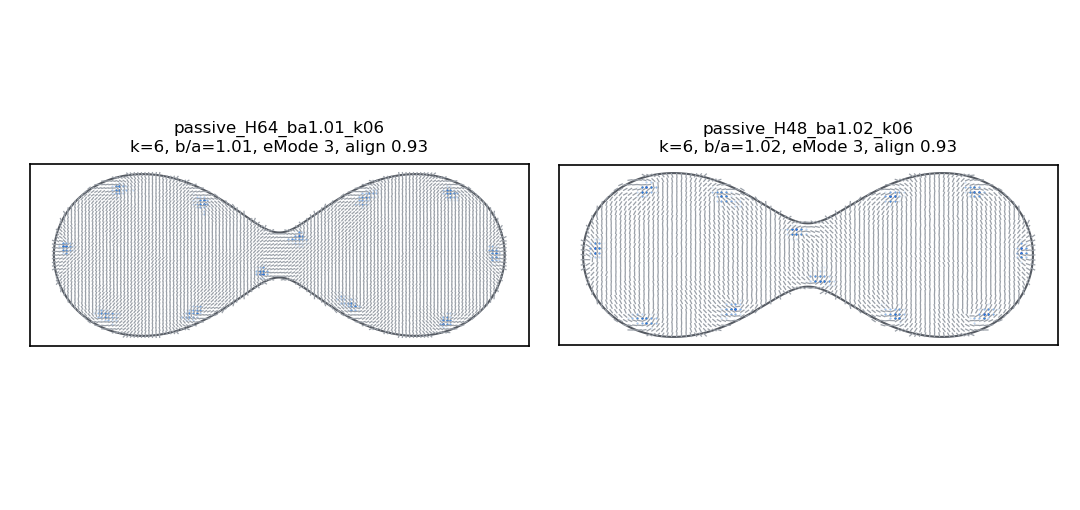
\includegraphics[width=\textwidth]{cassini_passive_pinched.png}
\caption{Passive pinched ovals ($b/a=1.02$ and 1.01, $k=6$): all imposed defects present and at the wall or in the neck.}\label{fig:passpinch}
\end{figure}
